\documentclass{article}

\usepackage{listings}
\usepackage{hyperref}
\usepackage{amsmath}
\usepackage{pgf}
\usepackage{tikz}
\usetikzlibrary{arrows,shapes,snakes,automata,backgrounds,petri,matrix,plotmarks,decorations.markings}
\usepackage{xcolor}
\usepackage[backend=bibtex]{biblatex} 
\addbibresource{bib/machine-learning}
\usepackage{leftidx}
\usepackage{mathrsfs}
\usepackage{appendix}




% For spec
\lstnewenvironment{spec}[1][]
{\lstset{ frame=tblr
		, #1%
	}%
	\csname lst@SetFirstLabel\endcsname}
{\csname lst@SaveFirstLabel\endcsname}

% For ghci
\lstnewenvironment{ghci}[1][]
{\lstset{ frame=tblr
		, literate={ghciLL>}{{$\,\lambda$>}}1%
		{ghciLL|}{{$\,\lambda$|}}1
		, #1%
	}%
	\csname lst@SetFirstLabel\endcsname}
{\csname lst@SaveFirstLabel\endcsname}

% For latex
\lstnewenvironment{latex}[1][]
{\lstset{ frame=tblr
		, language=LaTeX
		, #1%
	}%
	\csname lst@SetFirstLabel\endcsname}
{\csname lst@SaveFirstLabel\endcsname}

% for common
\lstset{
	breaklines,
	numbers=left,
	basicstyle=\small\ttfamily,
	flexiblecolumns=false,
	basewidth={0.5em,0.45em},
}



%%% datas5
\begin{filecontents}{knn.1.igndata}
    1  1
    2  3
    10 13
    20 18
    14 9
\end{filecontents}
\begin{filecontents}{knn.2.igndata}
    10  1
    20  3
    1  13
    2  18
    1  9
\end{filecontents}


\tikzstyle{arrow} = [ decoration={markings,mark=at position%
	1 with {\arrow[scale=3,>=stealth]{>}}},%
	double distance=1.5pt, black,shorten >= 3pt,%
	preaction = {decorate,black},%
	postaction = {draw,line width=2.5pt, black,shorten >= 3pt}]

\title{The Summary of Machine Learning}
\author{John Lee \\  me@qinka.pro \\ qinka@live.com}

\begin{document}
\maketitle
\begin{abstract}
  This report is mainly about basic algorithms for machine learning,
  including supervised classification, supervised regression, and unsupervised clustering.
  The mainly algorithms are decision tree, k-nearest negihbor, support vector machine, nerual network,
  linear-regression, k-means, hierarchial, and convolution nerual network.
  Most of these algorithms will be instanced with Haskell, and most of them are applied to NAO robot.
  All the codes and this report are opend on GitHub, with GNU's
  \href{https://www.gnu.org/copyleft/gpl.html}{GPLv3+} license and GNU's
  \href{https://www.gnu.org/licenses/quick-guide-gplv3.html}{FDL}.
\end{abstract}
\section*{Copyleft}
\label{sec:copyleft}

All of these codes and documents are under GNU's GPLv3+ and FDLv1.3+. \\
{\large Copyleft (C) 2017 John Lee <me@qinka.pro> <qinka@live.com>} \\

\paragraph{Notice for Codes}

All the codes in the reimagined-pancake are under GPLv3+ license.

Reimagined-Pancake is a serial toy about machine learning and NAO robot.
Copyright (C) 2017 John Lee <me@qinka.pro> <qinka@live.com>

This program is free software: you can redistribute it and/or modify
it under the terms of the GNU General Public License as published by
the Free Software Foundation, either version 3 of the License, or
(at your option) any later version.

This program is distributed in the hope that it will be useful,
but WITHOUT ANY WARRANTY; without even the implied warranty of
MERCHANTABILITY or FITNESS FOR A PARTICULAR PURPOSE.  See the
GNU General Public License for more details.

You should have received a copy of the GNU General Public License
along with this program.  If not, see \href{http://www.gnu.org/licenses}{<http://www.gnu.org/licenses/>}.

\paragraph{Notice for Documents and Reports}

In reimagined-pancake, all the documents(not including the one in the codes), reports and other texts,
are under the GNU's FDLv1.3+ license.

This report is a summary, or say a report about the machine.

Copyright (C)  2017 John Lee <me@qinka.pro> <qinka@live.com>

Permission is granted to copy, distribute and/or modify this document
under the terms of the GNU Free Documentation License, Version 1.3
or any later version published by the Free Software Foundation;
with no Invariant Sections, no Front-Cover Texts, and no Back-Cover Texts.
A copy of the license is included in the section entitled "GNU
Free Documentation License".

You should have received a copy of the GNU Free Documentation License
along with this program.  If not, see \href{http://www.gnu.org/licenses}{<http://www.gnu.org/licenses/>}.

\section{Machine Learning}
\label{sec:ml}

The machine learning is a serial of tasks to learning the unknown things with the known thing.
The commonly way of machine learning is that we use the known data, or say training data, and model whose parameters are unknown,
to predict those which we don't known well but will happen in the feature.  The core of learning is get the unknown parameters well.
For example, there are some points, which fit the linear model $y = wx+b$, and our goal is learning the parameter $w$ and $b$.

The machine learning mainly includes supervised classification, supervised regression, and unsupervised clustering.
For supervised classification, decision tree, knn, support vector machine, neural network are commonly used.
For supervised regression, support vector machine, ordinary least squares, are commonly used.
For unsupervised clustering, the k-means, and hierarchical clustering are commonly used.

\section{Decision Tree}
\label{sec:decisiontree}

For the first algorithm about machine learning, let's talk about decision tree.

The decision tree is just like a state machine or flow chart, and it is a like of decision support tool
by using a tree-like graph or model to help people make decision, while it can also help machine.

The way it works is that in the each node, there is a if-condition, and when it's true it will move to
one of sub-node. When it's false, it will move to another sub-node. When it moves to the end-node,
that means there is a decision which we can make.

For example, if you want to know whether you need to take an umbrella, the ``if-condition'' is
whether it's raining outside. If the condition is true, you need to move to end-node, ``take an umbrella'',
and if not, you need to move to the end-node, ``leave umbrella alone''.
If it's drawn as a graph, it will likely be figure\ref{fig:dt:eg}.

\begin{figure}
  \centering
  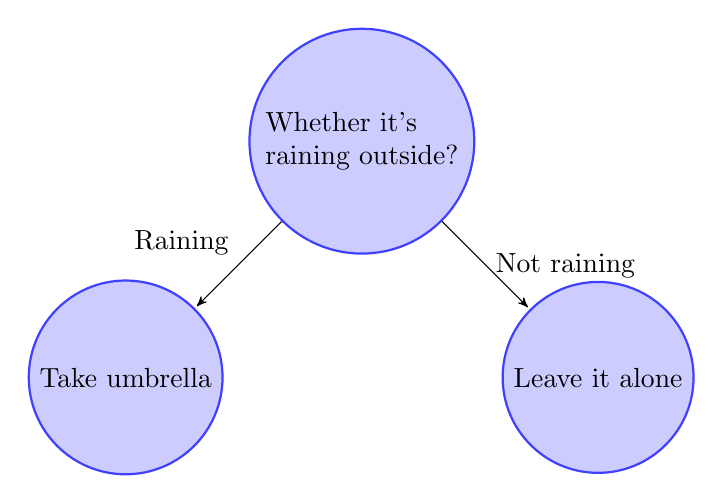
\begin{tikzpicture}[node distance=3cm,>=stealth',bend angle=20,auto]        
    \tikzstyle{point}=[circle,thick,draw=blue!75,fill=blue!20,minimum size=6mm]
    \begin{scope}
      \node[point](rain){\vbox{\hbox{Whether it's}\hbox{raining outside?}}};
      \node[point,below of=rain,left of=rain](take){Take umbrella}
      edge [pre] node {Raining} (rain);
      \node[point,below of=rain,right of=rain](leave){Leave it alone}
      edge [pre,right] node {Not raining} (rain);
    \end{scope}
  \end{tikzpicture}
  \caption{The decision tree for example.}
  \label{fig:dt:eg}
\end{figure}

\subsection{How Does Machine Learning?}
\label{sec:dt:how}

First of all, we need to know what entropy is.
Then we will talk about ID3 algorithm to learning a decision tree.

\subsubsection{Entropy}
\label{sec:dt:how:entropy}

Entropy was defined to represent the ``size'', or say amount of informations.
Simply, it represent how many bit are needed to encode a serial of informations.
The equation of the entropy is equation.\ref{eq:entroy}.
\begin{equation}
  \label{eq:entropy}
  H(X) = - \sum\limits_x P(x)\log_2\left[P(x)\right]
\end{equation}
And that means the entropy will be larger when the variable's more uncertain.
The unit of entropy is bit.

For example, there is an asymmetrical coin. The probability of frontage is 0.8,
while that of other size is 0.2.
So the entropy is $H(X) = - 0.2\log_20.2 - 0.8\log_20.8 = 0.7219$.

\subsubsection{ID3}
\label{sec:dt:how:id3}

When there are many attributes which can be used as ``if-condition'',
we need to find out one of them as the node. So the information gain is defined.
\begin{equation}
  \label{eq:inforgain}
  Gain(A) = Info(D) - Info_A(D)
\end{equation}
where $A$ means one of the attributes, and $Info$ means simply entropy.
The $Info_A$ means the average entropy for each range of age.
The difference means how many informations we can ``get'' if ``split'' by age.

So the basic idea of ID3 algorithm is 
\begin{quote}
  For each node, find out which attribute's \textit{information gain} is the largest.
  If there is not any attribute or all item in this node belongs to one class, this node is a end-node.
  If there is a attribute's information gain is the largest, the tree will be split by this attribute.
  And then do it again until we get all the end-node.
\end{quote}

\section{K-Nearest Neighbor}
\label{sec:knn}

K-Nearest Neighbor uses distence to classify. For an item, the k-nearest neighbors will be use
to classify.
For example, in the figure \ref{fig:knn:eg}, when the $k=2$, the item should be same with white one.
\begin{figure}
	\centering
	\begin{tikzpicture}[only marks, y=.3cm,x=.3cm]
	%axis
	\draw (0,0) -- coordinate (x axis mid) (22,0);
	\draw (0,0) -- coordinate (y axis mid) (0,22);
	\draw plot[mark=*,mark options={fill=white}] file {knn.1.igndata};
	\draw plot[mark=*] file {knn.2.igndata};
	\draw plot[mark=square*, mark options={fill=white}] (10,10);
	\draw [dashed] (10,10) circle [radius=5];
	\end{tikzpicture}
	\caption{Example of k-NN classifcation, where k = 2}
	\label{fig:knn:eg}
\end{figure}

\subsection{How to learning?}
\label{sec:knn:learning}

The first step is computing the distances between item, which need to be classified, and training datas.
The second step is finding out which class the most of k-nearest neighbors belong to.

Normally, we can use \textbf{euclidean distance}, \textbf{cosine}, \textbf{correlation},
or \textbf{manhattan distance} to measure the distance.

\subsection{Example of Codes}
\label{sec:knn:code}

\section{Support Vector Machine}
\label{sec:svm}

Support vector machines are supervised learning models\cite{svm-wikipedia}. It's mainly used to classify,
while it can also be use to regression analysis.
The basic ideas of support vector machine are
\begin{itemize}
\item Mapping data to higher-dimensional linear-separable feature space
\item Finding out the best hyperplane to split data
\end{itemize}

\subsection{Kernel Function}
\label{sec:svm:kf}

To map the samples to the feature space, there are many ways to do it.
However, it is possible that samples are mapped to a infiniet-dimensional space.
For example, we can use $\phi(x)=(1,x,x^2,x^3,\dots)^T$ to map samples to a infiniet-dimensional space.
But that is bad idea, because it is impossible to compute.
So we need to use kernel function to map.

So let me tell you how to use kernel function.
The kernel function is dualistic function $K(\cdot,\cdot)$.
For samples $\{(\mathbf{x}_i,y_i)\}^n_{i=1}$, and kernel function(s) $K(\mathbf{x},\mathbf{x}_j)^n_{j=1}$,
the mapping function\cite{GraphML1} will be defined as
\begin{equation}
  \label{eq:mapping}
  f_\theta(\mathbf{x})=\sum\limits_{j=1}^{n}\theta K(\mathbf{x},\mathbf{x}_k)
\end{equation}
There are some popular kernel function:
\begin{itemize}
\item linear
  \begin{equation}
    \label{eq:kf:linear}
    K(\mathbf{x}_i,\mathbf{x}_j) = \mathbf{x}_i^T\mathbf{x}_j
  \end{equation}
\item polynomial
  \begin{equation}
    \label{eq:kf:polynomial}
    K(\mathbf{x}_i,\mathbf{x}_j) = \left(\gamma \mathbf{x}_i^T\mathbf{x}_j+r\right)^d,\gamma > 0
  \end{equation}
  %% 径向基函数
\item radial basis function
  \begin{equation}
    \label{eq:kf:rbf}
    K(\mathbf{x}_i,\mathbf{x}_j) = \exp{\left(-\gamma||\mathbf{x}_i-\mathbf{x}_j||^2\right)},\gamma > 0
  \end{equation}
\item sigmoid
  \begin{equation}
    \label{eq:kf:sigmoid}
    K(\mathbf{x}_i,\mathbf{x}_j) = \tanh{\left(\gamma \mathbf{x}_i^T\mathbf{x}_j+r\right)}
  \end{equation}
\end{itemize}
where $\gamma$,$r$, and $d$ are kernel parameters.

\subsection{Hyperplane}
\label{sec:svm:hyperplane}

The hyperplane used to classify should have the largest distances to it's nearest training-data.

So, one of model to represent hyperplane is:
$$
\mathbf{x} = \left[\begin{array}{c} x_1 \\ x_2 \\ \vdots \\ x_d \end{array}\right];
\mathbf{w} = \left[\begin{array}{c} w_1 \\ w_2 \\ \vdots \\ w_d \end{array}\right];
h(\mathbf{x}) = sign\left(\mathbf{w}^T\mathbf{x}+b\right)
$$
It is, at the same times, also a optimization problem, and the model\cite{svm1} is:
\begin{equation}
\label{eq:hyp:op}
\begin{array}{rl}
  \min\limits_{\mathbf{w},b,\mathbf{\xi}} & \frac{1}{2}\mathbf{w}^T\mathbf{w}+C\sum\limits_{i=1}^{l}\xi_i\\
  \text{subject to} & y_i\left(\mathbf{w}^T\phi(\mathbf{x}_i)+b\right) \geq 1 - \xi_i,\\
                                          & \xi_i \geq 0.
\end{array}
\end{equation}

\subsection{How to learn?}
\label{sec:svm:how}

The best way to find out that hyperplane is find the solution of that optimization problem.
By using Lagrange multiplier method\cite{GraphML1}:
\begin{equation}
  \label{eq:lagrange-multiplier-method}
  L(\mathbf{\omega},\gamma,\mathbf{\xi},\mathbf{\alpha},\mathbf{\beta}) =
  \frac{1}{2}\parallel\mathbf{\omega}\parallel^2+C\sum\limits_{i=1}^{n}\xi_i
  - \sum\limits_{i=1}^{n}a_i\left(\left(\mathbf{\omega}^T\mathbf{x}_i+\gamma\right)y_i-1+
  xi_i\right) - \sum\limits_{i=1}^{n}\beta_i\xi_i
\end{equation}
And that is equal to:
\begin{equation}
\max\limits_{\mathbf{\alpha},\mathbf{\beta}}\inf\limits_{\mathbf{\omega},\gamma,\mathbf{\xi}}
 L(\mathbf{\omega},\gamma,\mathbf{\xi},\mathbf{\alpha},\mathbf{\beta})
\end{equation}
subjects are $\mathbf{\alpha} \geq 0,\mathbf{\beta} \geq 0$.
Because of the optimized condition of $\inf{\mathbf{\omega},\gamma,\mathbf{\xi}}
L(\mathbf{\omega},\gamma,\mathbf{\xi},\mathbf{\alpha},\mathbf{\beta})$,
there are
$$\begin{array}{ccccl}
\frac{\partial L}{\partial \mathbf{\omega}} & = & 0 & \Rightarrow & \mathbf{\omega} = \sum\limits_{i=1}^{n}\alpha_iy_i\mathbf{x}_i \\
\frac{\partial L}{\partial \gamma} & = & 0 & \Rightarrow & \sum\limits_{i=1}^{n}\alpha_iy_i = 0 \\
\frac{\partial L}{\partial \xi_i} & = & 0 & \Rightarrow & \alpha_i + \beta_i = C, \forall i=1,\dots,n
\end{array}
$$

So finally the values of parameters can be learned:
\begin{align}
\hat{\mathbf{\alpha}} &= \mathop{argmax}_\alpha\left[\sum\limits_{i=1}^{n}\alpha_i-\frac{1}{2}\sum\limits_{i,j=1}^{n}\alpha_i\alpha_jy_iy_j\mathbf{x}^T_i\mathbf{x}_j \right]
\\
\hat{\mathbf{\omega}} &= \sum\limits_{i=1}^{n}\hat{\alpha_i}y_i\mathbf{x}_i
\\
\hat{\gamma} &= y_i - \sum\limits_{j:\hat{\alpha}_i>0}\hat{\alpha}_iy_i\mathbf{x}_i^T\mathbf{x}_j
\end{align}


\section{Nerual Network}
\label{sec:nn}

In deep learning, nerual networks is the important things.
The neural network is a kind of ``model'' which can present how human's brain work.
Human's brain is a high performance parallel computer, for people can deal with complex images\cite{NNnML1}.
So some one%
\footnote{Warren McCulloch and Walter Pitts(1943),\cite{McCulloch194}}
created model: artificial neural network.

The figure \ref{fig:nn} is an example for neural network.
There are two main elements: node(neuro) and link(cynapes).
When a serial of data ``passing-by'' a neuro, there are two events which will happen.

Let $\mathbf{x}_i$ be the input of layer $i$ in the neural network, let $\mathbf{w}_i$
be the weight of the cynapes between the layer $i$ and layer $i+1$,
and let $\mathbf{b}_i$ be the biases for this layer's neuros.
So the next level's input, or say this layer's output will be
$$
  O = \phi\left(\mathbf{x}_i\mathbf{w}_i + \mathbf{b}_i\right)
$$
where $\phi(\cdot)$ is an activation function, e.g. sigmoid function.
With the inputs, the neural network can approximate the linear or -non-linear functions:
\begin{equation}
  \label{eq:nn:app}
  \begin{array}{rcl}
  f(\mathbf{x}) &=& ^nf_{\mathbf{w}_n,\mathbf{b}_n}(\mathbf{x}) \\
  {}^if_{\mathbf{w}_i,\mathbf{b}_i}(\mathbf{x}) &=& \phi\left({}^{i-1}\mathbf{f}_{\mathbf{w}_{i-1},\mathbf{b}_{i-1}}(\mathbf{x})\mathbf{w}_i + \mathbf{b}_i\right)
  \end{array}
\end{equation}

\subsection{How Do Machines Learn?}
\label{sec:nn:how}

The way to learn $\hat{f}$ is using gradient descent and backpropagation.
For a neural network $f(\cdot)$, its paramters include weight($\mathbf{w}_i$),
and bias($\mathbf{b}_i$) for each neuro. So for each time of training, 
let $\Delta$ be
$$
 f(\mathbf{x}_i) - \hat{f}(\mathbf{x}_i)
$$
and then for each layer's parameters the updatings can be worked out:
\begin{align*}
  \Delta w_{ij} = l{Err_jO_j} \\
  \Delta b_{ij} = l{Err_j}
\end{align*}
where $Err_j$ is $O_j(1-O_j)(T_j-O_j)$(for output layer) or $O_j(1-O_j)\sum\limits_kErr_kw_{jk}$(for hidden layer).


\section{Linear Regression}
\label{sec:lreg}

For linear regression, there we use the gradient descent.
For a linear model $y=\mathbf{w}\mathbf{x}+\mathbf{b}$, we use the following method to training.
And we use the $\theta$ to present the $\mathbf{w}$ and $\mathbf{b}$.

First, we need  to define the loss function
\[
loss_\theta = \alpha(\hat{y}_\theta - y)^2
\]
So the gradient is
\begin{align*}
\nabla &= \frac{\partial}{\partial \theta}loss_\theta \\
       &= 2\alpha (\hat{y}_\theta -y)\cdot \frac{\partial}{\partial \theta}\left(\theta \mathbf{x} - y\right) 5 \\
       &= 2\alpha(\hat{y}_\theta -y)\mathbf{x}
\end{align*}
where if let $\alpha$ be $\frac{1}{2}$, the $2$ will be divided out.
Then we update the parameter $\theta$:
\[
\theta = \theta - \eta\nabla
\]
where the $\eta$ means the ratio of learning, and in other words, that means length of step.

\subsection{Linear Learning}
\label{sec:lreg:how}

Now, we can learning parameters with the aboves method.
If the $x$ is scalar, the $w$ and $b$ will also be scalar. If $\mathbf{x}$ is not scalar, or say is vector,
we can just the $\phi(\cdot)$ to ``represent'' the more complex function.
So the function will be 
\[
y(x) = \mathbf{w}\phi_n(x)
\]
If there is $\phi(x)_n = (1,x,x^2,\dots,x^n)^T$, that will polynomial one, and it also can be $\phi(x)_n = (1,\cos(x),\cos(2x),\dots,\cos(nx)^T$.
And the regression will still be linear.

\section{K-Means}
\label{sec:kmeans}

K-Means is an unsupervised clustering learning method. Its core idea is recompute a category's central point, in the feature map,  according
to the old classification.

\subsection{How does it work?}
\label{sec:kmeans:how}

There two status for learning machine: initialization, and new data passed in.
For the initialization, the central point of classes, should be chosen well.
When a new data coming in, we should do
\begin{itemize}
	\item Use old classification to classify the new data.
	\item Use some method to compute new central point of each category, and recompute the class of each point.
\end{itemize}

\section{Hierarchical Clustering}
\label{sec:hc}

It is a little like Huffman coding. The basic idea is finding out the two nearest point in the feature space, and merge them to ``one'', and then redo.

\subsection{How does it work?}
\label{sec:hc:how}

For those points in the feature space, first step is finding out the nearest two points, and merge them to a class.
Then do it again and again until there are only one class. 

\section{Gradient Descent}
\label{sec:gd}

Gradient descent is an algorithm to find out the local minimum of a function. For those functions who have a local minimum,
the ``point'', in the space, will be moved in the step of gradient.
For a multi-variable function $F(\mathbf{x})$, which is defined and differentiable at the point $\mathbf{\alpha}$, 
the fastest-decreases at point $\mathbf{\alpha}$ is at the direction of $-\nabla F(\mathbf{\alpha})$.
And the next point in the space should be
\begin{equation}
	\label{eq:gd:next}
	\mathbf{\alpha}^{n+1} = \mathbf{\alpha}^n - \eta\nabla F(\mathbf{\alpha}^n)
\end{equation}
In the machine learning, the $\gamma$ is called learning rate. When we computing the differential, the $\gamma$ usually is $\lim\limits_{x \rightarrow \infty} \frac{1}{x}$

For example, let $F(x_1,x_2)=w_1e^{w_2x_1}+w_3\ln(w_4+x_2)$. So the updating for $x_1$ and $ x_2$ will be 
\begin{align*}
x_1^{i+1} &= x_1^i - \eta\nabla F(x_1^i) \\ &= x_1^i - \eta w_1w_2e^{2_2x_1} \\
x_2^{i+1} &= x_2^i - \eta\nabla F(x_2^i) \\ &= x_2^i -\eta w_3\frac{1}{w_4+x_2}
\end{align*}

\subsection{Stochastic Gradient Descent}
\label{aec:gd:sgd}

Stochastic gradient descent, SGD for short, use stochastic approximation in gradient descent optimization method.

For example, when we use the gradient descent to regress a linear function $f(x) = wx+b$, and we have batches of training data.
If your size of batch is about 100, and the loss function is
\[
\ell = (\hat{(f)} - f)^2
\]
the updating for $w$ and $b$(using $|theta$ to present parameters) will be
\[
\tilde{\theta} = \theta - \frac{\eta}{m}\sum\limits_{i=1}{m}\nabla f_i(w)
\]
When the size of batch larger enough, about million, the size cost on computing will be much more.
So the stochastic approximation method is imported to gradient descent. Though the direction of descent of each time is not
the fastest one, but the SGD do speed up the solving
\[
\tilde{\theta} = \theta - \eta _i\nabla f_i(w_i)
\]

\subsection{Gradient Descent Optimization Algorithms}
\label{sec:gd:gdoa}

So in the following, we will outline some of the algorithms about gradient descent optimization. The main part of the following come from
\cite{DBLP:journals/corr/Ruder16} and \cite{wikipedia:sgd}. However, I just want to given you a snapshot.

\subsubsection{Momentum}
\label{sec:gd:gdoa:momentum}

The basic idea is that the updating in this time will include the ``information'', or say the descent of the last time.
In other words, the ``descent'' is related to this time's gradient, and the last time's
\[
\theta_{i+1} = \theta_i - \eta\left(\gamma\nabla_{i-1}J(\theta_{i-1}) + \nabla_iJ(\theta_i)\right)
\]
where $\gamma$ is a fraction of last time's updating.

\subsubsection{Nesterov Accelerated Gradient}
\label{sec:gd:gdoa:nag}

%% todo there are many gd should be talked about.

\section{Cross Entropy Cost}
\label{sec:cec}

Cross entropy between probability distributions: $p$, and $q$, which is under the same set of events, measures the average
the size of bits, which are needed to identify an event drawn from that set.
The equation of the cross entropy for $p$ and $q$ as:
\[
H(p,q) = E_p\left[-\log{q}\right] = H(p) + D_{KL}(p\\parallel q)
\] 
where $H(\cdot)$ represents the entropy, and $D_{KL}(\cdot)$ is the Kullback-Leibler divergence%
\footnote{ Kullback-Leibler divergence
	\[
	D_{KL}(p\parallel q) = \sum\limits_{x \in X}p(x)\log\frac{p(x)}{q(x)}
	\]
}.

For some reasons, the speed of learning with loss function $\ell = (\hat{y}-y)^2$ is not as fast as we wish.
So we use the cross entropy lost function
\[
\ell = - y\ln{\hat{y}}-(1-y)\ln{(1-\hat{y})}
\]
The partial derivative of parameter $\theta$ for $\ell$ is 
\[
\frac{\partial \ell}{\partial \theta} = - \frac{y}{\hat{y}}\frac{\partial\hat{y}}{\partial\theta} + \frac{1-y}{1-\hat{y}}\frac{\partial\hat{y}}{\partial \theta}
\] 
Then we can use gradient descent to updating our parameters.


\section{Backpropagation}
\label{sec:bp}

The backpropagation algorithm is an important method to update artificial neural network's parameter. 

For neural network's complex structure, using gradient descent some times is a trouble, because
compute the gradient is not easy. So we use the backpropagation to compute.

For a node $y$, which pass its output to ``next'' level as input,
if let the weights of the ``passings'' to next level be $w_i$, the 
loss of this node $\nabla y$ should be $\sum\limits_{i}w_i\nabla y$.
Just like figure \ref{fig:bp:1}.

\begin{figure}
    \centering
    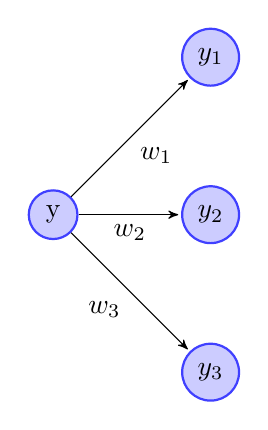
\begin{tikzpicture}[node distance=2cm,>=stealth',bend angle=20,auto]        
    \tikzstyle{point}=[circle,thick,draw=blue!75,fill=blue!20,minimum size=6mm]
    \begin{scope}
    \node[point](y){y};
    \node[point,right of=y,above of=y](y1){$y_1$}
    edge [pre] node {$w_1$} (y);
    \node[point,right of=y](y2){$y_2$}
    edge [pre] node {$w_2$} (y);
    \node[point,right of=y,below of=y](y3){$y_3$}
    edge [pre] node {$w_3$} (y);
    \end{scope}
    \end{tikzpicture}
    \caption{Backpropagation}
    \label{fig:bp:1}
\end{figure}


\section{Softmax}
\label{sec:softmax}

Softmax function is a generalization of the logistic function.
The input of softmax is a K-dimensional vector $\mathbf{z}$,
while the output, just as a logistic function, is a K-dimensional vector,
which range from 0 to 1. More, the sum of output is 1.
\begin{equation}
\sigma(\mathbf{z})_j = \frac{e^{z_j}}{\sum_{k=1}^{K}e^{z_k}}
\end{equation}
where $i \in 1,2,\dots,K$.
The softmax function can ``replace'' the sigmoid function in the neural network.


\section{Overfitting}
\label{sec:of}

When we try to fit our model to the training data, there are kinds of ``xx-fitting''. One is underfitting, and another is overfitting
One example of underfitting  is using linear model to fit a non-linear data.
This section will mainly talk about the overfitting. 

Firstly, let $\varepsilon$ be the error or say noise for the data, and let $\delta$ be the ``change'' of the function fitted to data.
So let's think about the $\varepsilon$ and $\delta$. When $\frac{\delta}{\varepsilon} \rightarrow 0$, we can say the error or noise of data has
very a little or even no influence to the function. If it overfitting, $\frac{\delta}{\varepsilon}$ will be a constant number of even $\infty$.

When the error or say noise has a obvious influence to function, the overfitting will happen.


\section{Convolutional Neural Network}
\label{sec:cnn}

The convolutional neural network, CNN for short, is an important method and is widely used in the deep learning.
CNN is mainly applied to analyzing the visual imagery. It can translate, or say transform, the images in  form of some color model, such as RGB,
to a rich feature or informations.
\begin{figure}
	\centering
	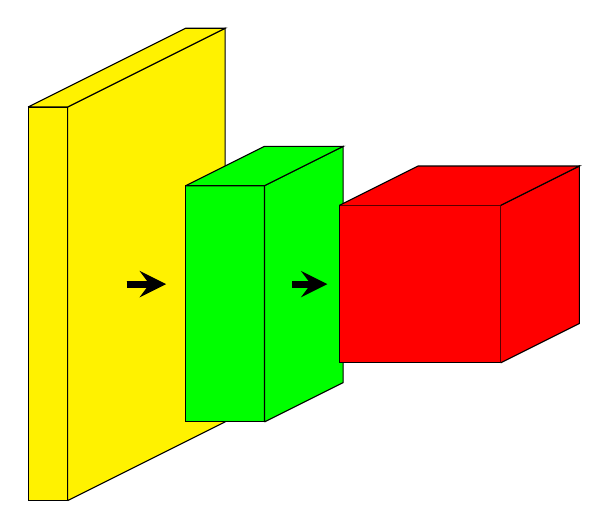
\begin{tikzpicture}[scale = .5]
		\fill[fill=yellow,draw=black] (0,0) -- (1,0) -- (1,10) -- (0,10) -- (0,0);
		\fill[fill=yellow,draw=black] (1,0) -- (5,2) -- (5,12) -- (1,10) -- (1,0);
		\fill[fill=yellow,draw=black] (0,10) -- (4,12) -- (5,12) -- (1,10) -- (0,10);
		\draw[arrow] (2.5,5.5) -> (3.5,5.5);
		\fill[fill=green,draw=black] (4,2) -- (6,2) -- (6,8) -- (4,8) -- (4,2);
		\fill[fill=green,draw=black] (6,2) -- (8,3) -- (8,9) -- (6,8) -- (6,2);
		\fill[fill=green,draw=black] (4,8) -- (6,9) -- (8,9) -- (6,8) -- (4,8);
		\draw[arrow] (6.7,5.5) -> (7.6,5.5);
		\fill[fill=red,draw=black] (7.9,3.5) -- (12,3.5) -- (12,7.5) -- (7.9,7.5) -- (7.9,3.5);
		\fill[fill=red,draw=black] (12,3.5) -- (14,4.5) -- (14,8.5) -- (12,7.5);
		\fill[fill=red,draw=black] (7.9,7.5) -- (9.9,8.5) -- (14,8.5) -- (12,7.5);
	\end{tikzpicture}
	\caption{The transformation of CNN}
	\label{fig:cnn:trans1}
\end{figure}
Usually, CNN will transform the a 3-channel(for colors) image($h\times w$) into a multi-channel small image.
For example, in figure \ref{fig:cnn:trans1}, the transformation increases the number of channel,
but shrink the image's size. That can help us extract the informations and features of image.

At the same time, a CNN layer includes
\begin{description}
	\item[Convolutional sublayer] This sublayer is the core of CNN. It do the convolution.
	\item[Pooling sublayer] Simply to say, this sublayer help us to shrink the size of image.
	\item[ReLU sublayber]  $f(x) = max(0,x)$
\end{description}

\begin{appendix}
	\newcounter{codeline}
	\setcounter{codeline}{1}
	\setcounter{lstnumber}{1}
	\lstnewenvironment{code}[1][]
	{ \setcounter{lstnumber}{\value{codeline}}
		\lstset{ numbers=left%
			, firstnumber=last%
			, literate={+}{{$+$}}1 % plus
			{/}{{$/$}}1
			{*}{{$*$}}1
			{=}{{$=$}}1
			{>}{{$>$}}1
			{<}{{$<$}}1
			{\\}{{$\lambda$}}1
			{\\\\}{{\char`\\\char`\\}}1
			{->}{{$\rightarrow$}}2
			{>=}{{$\geq$}}2
			{<-}{{$\leftarrow$}}2
			{<=}{{$\leq$}}2
			{=>}{{$\Rightarrow$}}2
			{\ .}{{$\circ$}}2
			{\ .\ }{{$\circ$}}2
			{>>}{{>>}}2
			{>>=}{{>>=}}2
			{|}{{$\mid$}}1
			{/=}{{$\neq$}}1
			, #1%
		}%
		\csname lst@SetFirstLabel\endcsname}
	{ \csname lst@SaveFirstLabel\endcsname
		\setcounter{codeline}{\value{lstnumber}}
	}
	
	\section{Codes Instance}
	\label{apdx:codes}
	
	This section is about the instance of the algorithms and ``toys''.
	All this codes are under the  GPLv3+.
	The intro. for running these codes are in the appendix \ref{apdx:run}.	
	%\lstinputlisting[lanuage=haskell,]{filename}
	
	\subsection{The Example for Decision Tree}
	\label{code:dc}
	
	The following is an instance in Haskell of decision tree with ID3 algorithm.
	\input{../decision-tree/decision-tree/src/AI/DecisionTree/ADT.lhs}
	\input{../decision-tree/decision-tree/src/AI/DecisionTree.lhs}
	
	\subsection{The Example for  K-Nearest Neighbor}
	\label{code:knn}
	
	The follwing is the instance in Haskell of k-nearest neighbor algorithm.
	\input{../knn/src/AI/KNN.lhs}
	
	\subsection{The Example of Using LIBSVM with Haskell}
	\label{code:svm}
	
	The following is the instance of using \href{https://www.csie.ntu.edu.tw/~cjlin/libsvm/index.html}{LIBSVM} in Haskell, with bindings:
	\href{https://github.com/aleator/Simple-SVM}{Simple-SVM} and \href{https://github.com/delanoe/bindings-svm}{bindings-svm}%
	\footnote{For these two binding, I just forked my bindings, and adjust for LibSVM-3.22. The url are \url{https://github.com/Qinka/Simple-SVM} and \url{https://github.com/Qinka/bindings-svm}.}.
	
	The following is the simple example, the model trained via libsvm's tool. The program just uses the well-trained model.
	\lstinputlisting[language=haskell]{../toy-backend/toy-backend-classify/src/svm/Toy/Backend/Classify.hs}\setcounter{codeline}{1}
	
	\subsection{The Example for Neural Network}
	\label{code:nn}
	
	The following codes is an example of using neural network to train a judger of human face.
	It works with tensorflow,
	\input{../nn/neural-network/src/AI/NN.lhs}\setcounter{codeline}{1}
	
	\subsection{The Example for Linear Regression}
	\label{code:lr}
	
	The following codes are the one using linear-regression with gradient descent.
	It can fit the model $y = \mathbf{w}\mathbf{x} + \mathbf{b}$, and also $y = \mathbf{w}\phi(\mathbf{x})+\mathbf{b}$.
	\input{../regress/src/AI/Regress/Internal.lhs}\setcounter{codeline}{1}
	\input{../regress/src/AI/Regress/Linear.lhs}\setcounter{codeline}{1}
	\input{../regress/src/AI/Regress/QuadraticCurve.lhs}\setcounter{codeline}{1}
	
	\subsection{The Example for MNIST}
	\label{code:mnist}
	
	The following codes are the example of MNIST, which can be used to recognize the handwritten numeral.
	\input{../nn/mnist/src/AI/MNIST.lhs}\setcounter{codeline}{1}
	
	\subsection{Toy for NAO Robot}
	\label{code:nao}
	
	
	
	\section{Running Codes}
	\label{apdx:run}
	
	This section is about the ``how'' for running these examples, and ``toys''.
	Most of them are written in Haskell. So if you want to running them, there are some things
	you need to do:
	\begin{enumerate}
		\item Install \href{https://www.haskell.org/ghc}{Glorious Glasgow Haskell Compilation System}
		\item Inatsll \href{https://www.haskellstack.org}{haskell-stack} or \href{https://www.haskell.org/cabal/}{haskell-cabal}
		\item Tensorflow library. For details, you can catch up with Tensorflow official install guides(for C).
	\end{enumerate}

	All these codes work well with GHC-8.0.2 and stackage nightly-2017-07-25.
	The docker images are available on the Docker Hub%
	\footnote{For some reason, the example of mnist is still unavailable.}.
	
	\subsection{Decision Tree}
	\label{run:dt}
	
	So here I will show you how to run this example.
	
\end{appendix}


\printbibliography
\tableofcontents
\end{document}